% Controller state machine. Build: make diagrams
\documentclass[tikz,border=6pt]{standalone}
\usepackage{lmodern}\renewcommand{\ttdefault}{cmtt}
\usetikzlibrary{positioning,arrows.meta,calc}
\DeclareRobustCommand{\code}[1]{\texttt{\detokenize{#1}}}
\tikzset{
  blk/.style={draw,rounded corners=2pt,align=center,minimum height=0.85cm,minimum width=2.1cm,fill=gray!8,font=\scriptsize},
  st/.style={draw,circle,align=center,minimum size=1.35cm,inner sep=1pt,fill=gray!8,font=\scriptsize},
  ar/.style={-{Stealth[length=2mm]},thick},
  lb/.style={font=\tiny,inner sep=1pt,fill=white}
}
\begin{document}
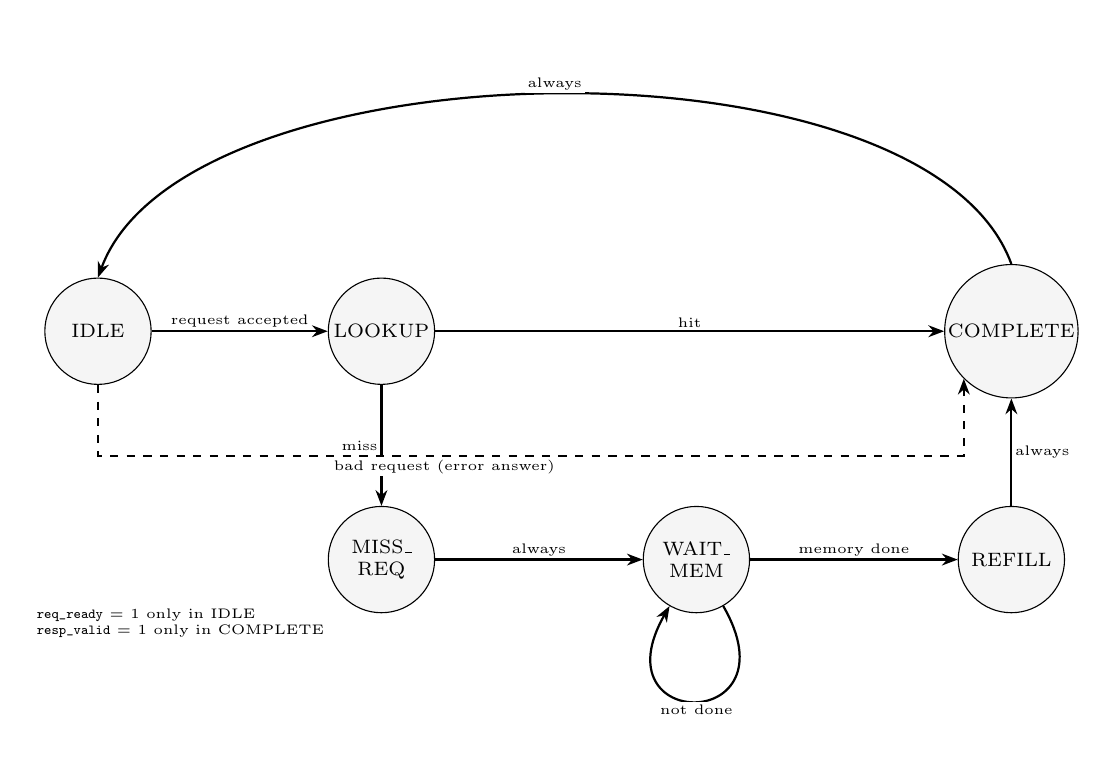
\begin{tikzpicture}[x=1cm,y=1cm]
  \node[st] (idle) at (0,0) {IDLE};
  \node[st] (look) at (3.6,0) {LOOKUP};
  \node[st] (comp) at (11.6,0) {COMPLETE};
  \node[st] (mreq) at (3.6,-2.9) {MISS\_\\REQ};
  \node[st] (wait) at (7.6,-2.9) {WAIT\_\\MEM};
  \node[st] (refl) at (11.6,-2.9) {REFILL};
  \draw[ar] (idle) -- node[lb,above]{request accepted} (look);
  \draw[ar] (look) -- node[lb,above]{hit} (comp);
  \draw[ar] (look) -- node[lb,left]{miss} (mreq);
  \draw[ar] (mreq) -- node[lb,above]{always} (wait);
  \draw[ar] (wait) -- node[lb,above]{memory done} (refl);
  \draw[ar] (refl) -- node[lb,right]{always} (comp);
  \draw[ar] (wait) to[out=-60,in=-120,looseness=7] node[lb,below]{not done} (wait);
  \draw[ar] (comp.north) to[out=110,in=70,looseness=0.7] node[lb,above]{always} (idle.north);
  \draw[ar,dashed] (idle.south) -- ++(0,-0.9) -| node[lb,pos=0.2,below]{bad request (error answer)} (comp.south west);
  \node[font=\tiny,align=left,anchor=north west] at (-0.9,-3.4) {\code{req_ready} = 1 only in IDLE\\\code{resp_valid} = 1 only in COMPLETE};
\end{tikzpicture}
\end{document}
